\documentclass{article}
\usepackage{amsmath}
%\usepackage{subfigure}
\usepackage{alltt}
\usepackage{verse}
\usepackage{subfig}
%\usepackage{wrapfig}
\usepackage{amsthm}
\usepackage{amssymb}
\usepackage{graphicx}
\usepackage{mdwlist}
\usepackage[colorlinks=true]{hyperref}
\usepackage{geometry}
\usepackage{titlesec}
\geometry{margin=1in}
\geometry{headheight=2in}
\geometry{top=2in}
\usepackage{palatino}
% \usepackage{mathrsfs}
\usepackage{fancyhdr}
\usepackage{paralist}
% \usepackage{todonotes}
\setlength{\marginparwidth}{2.15cm}
\usepackage{tikz}
\usetikzlibrary{positioning,shapes,backgrounds}
\usepackage{float} % Place figures where you ACTUALLY want it
\usepackage{comment}
\usepackage{ifthen}
\usepackage[]{mcode}
\rhead{}
\lhead{}

\renewcommand{\baselinestretch}{1.15}

% Shortcuts for commonly used operators
\newcommand{\E}{\mathbb{E}}
\newcommand{\Var}{\operatorname{Var}}
\newcommand{\Cov}{\operatorname{Cov}}
\DeclareMathOperator{\argmin}{arg\,min}
\DeclareMathOperator{\argmax}{arg\,max}

% do not number subsection and below
\setcounter{secnumdepth}{2}

% custom format subsection
\titleformat*{\subsection}{\large\bfseries}

% set up the \question shortcut
\newcounter{question}[section]
\newenvironment{question}[1][]
  {\refstepcounter{question}\par\addvspace{1em}\textbf{Question~\Alph{question}\!
    \ifthenelse{\equal{#1}{}}{}{ [#1 points]}: }}
    {\par\vspace{\baselineskip}}

\newcounter{subquestion}[question]
\newenvironment{subquestion}[1][]
  {\refstepcounter{subquestion}\par\medskip\textbf{\roman{subquestion}.\!
    \ifthenelse{\equal{#1}{}}{}{ [#1 points]:}} }
  {\par\addvspace{\baselineskip}}

\titlespacing\section{0pt}{12pt plus 2pt minus 2pt}{0pt plus 2pt minus 2pt}
\titlespacing\subsection{0pt}{12pt plus 4pt minus 2pt}{0pt plus 2pt minus 2pt}
\titlespacing\subsubsection{0pt}{12pt plus 4pt minus 2pt}{0pt plus 2pt minus 2pt}

\usepackage[]{mcode}


\chead{%
  {\vbox{%
      \vspace{2mm}
      \large
      Machine Learning \& Data Mining \hfill
      Caltech CS/CNS/EE 155 \hfill \\[1pt]
      Miniproject 2\hfill
      Math $10^{\text{th}}$, 2016 \\
    }
  }
}


\begin{document}
\pagestyle{fancy}

\LARGE
\begin{center}
CS 155 Miniproject 2: JustTryIt Team Report

\large
Kangchen Bai, Pengchuan Zhang, Yerong Li
\end{center}

\normalsize
\medskip

\section{Overview}
\paragraph{}
In the project, we work on the \textbf{Hidden Markov Model (HHM)} and the \textbf{Markov model} for poem generations. 

Due to the clear rhyme pattern in Shakespeare's sonnets, the basic strategy in our model training is to train multiple models for different part of the poem. We tokenize the words as features in each group and run the EM algorithm with different number of hidden states to train the HMMs. We developed several improvement techniques to get better poem generating performance: we train the HMM in the reverse direction and learn rhyme dictionary to sample last words that rhyme; we generate lines with total number of syllables as close to 10 as possible. With these techniques, we are able to generate poems which honor the rhyme pattern nor the iambic pentameter in Shakespeare's sonnets, and thus sound like Shakepeare's. We apply the same improvement techniques to train the Markov models as well.

The Hidden Markov Model is interesting due to the visualization and interpretation of hidden states. Looking into the model with 5 hidden states, we are able to find a clear relationship between the position of words and hidden states they correspond to. For more information, see Section \ref{sec:visualization}.

For Markov models, we pay special attention to the \textit{2nd Order Markov Model}. In comparison with the first-order Markov model, the 2nd-order Markov model turns out to be a better and more precise model in the task of poem generation. Since there are only, in total, around 3000 different words in Shakespeare's sonnets and we we trained in groups, the number of distinct words in each group is below 1000.

As additional goals, we work on data of Spenser's poetry set and we also work on the rhyme scheme in detail.


\section{Data Manipulation}
%
\vspace{5pt}
\paragraph{}
The basic strategy in our model training is to train multiple models for different part of the poem. Therefore, we have the following pre-processing data manipulation.

\begin{enumerate}
	\item [\textbf{Grouping}] Shakespear's sonnets enjoy the clear rhyme scheme \textit{abab cdcd efef gg}. Moreover, lines with different rhymes have quite different sentence structure. For example, the first and third lines \textit{aa} have quite different sentence structure from the last two lines \textit{gg}. Based on this obersevation, we decide to train 6 models for these 6 parts, namely \textit{a, b, c, d, e, f, g}. Therefore, we first group all the lines in the same part of the poems and get six corpuses, namely \texttt{groupA, groupB, groupC, groupD, groupE, groupF, groupG}.
	\item [\textbf{Punctuations}] Shakespear's sonnets contain various punctuations (e.g., `` ,", `` '", `` -"). We delete all punctuations except `` -", and thus the words ``Feed'st" and ``'This" become ``Feedst" and ``This". For words with hyphen `` -", we manually delete it or replace it with empty space ``  ". There are in total 83 hyphens in \texttt{Shakespear.txt} and it is very easy to deal with hyphens manually. After this stage, we have six corpuses and every corpus contains hundreds of lines without any punctuations. In poetry generation, we took our own punctuation scheme based on the writing style of Shakespeare's and our punctuations in each line of the poem are generated \textbf{automatically} by programs. 
	\item [\textbf{Tokenization}] We tokenize the words as features and use the method \texttt{text.CountVectorizer} from \texttt{sklearn.feature\_extraction} to preprocess every corpus. In simple, \texttt{CountVectorizer} lowercases all the words and builds a dictionary between the words and the natural numbers $\mathbb{N}$. The output of this tokenization step is six corpuses with sequences of natural numbers. These six corpuses will be the input of our model-training algorithms, e.g., HHM and 2nd-order Markov model.
\end{enumerate}

To achieve better poem-generating performance, we generate each line in the reverse direction with pre-sampled rhyming ending words. We keep generating lines until we get a line with exactly 10 syllables. In order to achieve these additional goals, we have the following pre-processing data manipulation.
\begin{enumerate}
	\item [\textbf{Generating rhyming dictionary}] We use the \textit{NLTK} package and the RhymeBrain website~\url{http://rhymebrain.com/en} to build a dictionary for rhyming words. For more details, see Section~\ref{sec:rhymedict}.{\color{blue}\ NEED SOME TEXT} Briefly summarize how we are using this dictionary.
	\item [\textbf{Counting syllables in each word}] We use the \textit{NLTK} package, the \textit{PyHyphen} package and our own-written function \texttt{count\_syllables()} to count the number of syllables in each word. These three methods have their own advantages and disadvantages, and we combine them to get the most accurate syllables-counting. For more details, see Section~\ref{sec:syllablecount}.
\end{enumerate}

\section{Unsupervised Learning}
We worked on Hidden Markov Model and Markov Model in this project.

%% subsection fo models
\subsection{Hidden Markov Model}
%
\paragraph{}
In training HMM, we tried on several number of hidden state in our model and chose the numjber of state with the highest emission probabilities as the favorate model in the project. To be specific, we tried on models with 5, 10, 20, 40, 80, and 100. We are working on model with 100 hidden states because there are around 3000 words in Shakespeare's poetry set and blow 1000 words for each group. In our training of Hidden Markov Model,  we maximal the emitting probability of the training set rather than minimizing the Frobenius norm of differeces in \textbf{transition matrix} and \textbf{observation matrix} for the simple reason that in this unsupervised training, the shape of transition matrix and observation matrix differs a lot : observation matrix has much more elements than transition matrix in most of the test cases, with number of hidden states 5, 10, and 20, for
instancce. So we maximize the emitting probability instead. Figure \ref{fig:probability} shows when the number of states increases of $\log P$ will increase accordingly. This is to say that choosing number of states according to emitting probability may not be good since if the number of state is too large, say, close to the number of words in each group, the hidden states themselves are not representative.
 \begin{figure}[ht!]
 \centering
 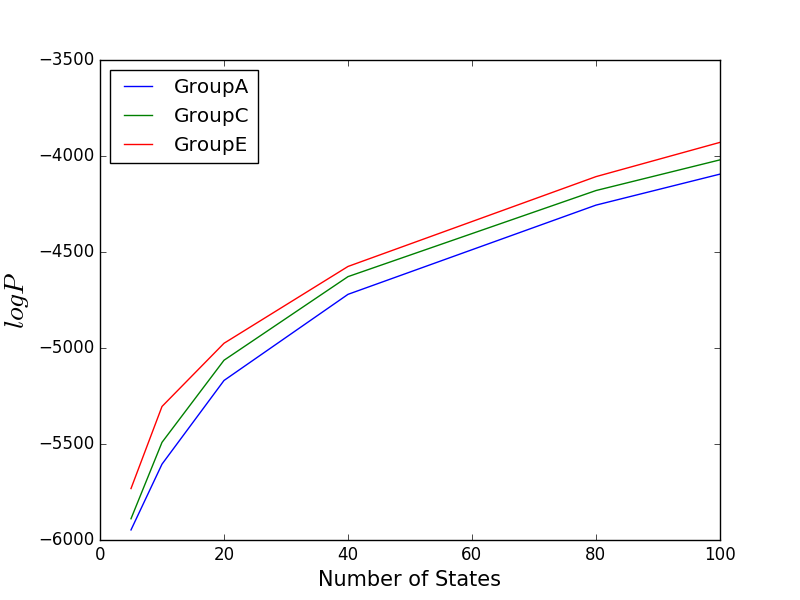
\includegraphics[width=0.6\textwidth]{./figure/probability.png}
 \caption{The emitting probability on training set \textit{Group A}, \textit{Group C} and \textit{Group E} the vertical axis is kept as $\log P$\label{fig:probability}}
 \end{figure}
\paragraph{The Optimal choice for the number of states} Usually, the way to choose the right number of hidden state is to do cross validation: train a model on one part of the corpus (training set) and calculate the emitting probability of the other half of the corpus (testing set) and choose the number that can maximize the emitting probability of the testing set.

\paragraph{}
However, since the fact that most of the words in the corpus appears only once, we abandon the cross validation approach. We choose the best hidden state number by inspecting the quality of the generated sentences. We decide that the larger the number is, the better the generated poem will be. We will elaborate this problem at a later section. 
\paragraph{Higher Model}
We also considered higher Markov model, but as a simple reason, higher order may not perform much better than the second order, in the poetry language, especially,we have usually taken 2 word as a phrase. And if the order of the model is too high, actually we may generate a whole line from the original data set, and that is not what we are expecting. 


\subsection{Markov Model}
%
\vspace{5pt}
\subsubsection{1st order Markov Chain Model}
\vspace{5pt}
\paragraph{\textit{The relationship between HMM and original Markov Chain Model}} We see in history that Hidden Markov Model is necessary when the number of observation states (number of words in Shakespeare's Sonnets, in this case) is unavoidable large. Besides this, we need Hidden Markov Model because we are supposed to get some intuitions in the grouping of words and hidden states are bringing us information. But in the case that the number of different words is affordably large (there are around 3000 words in this case), Markov Chain proves a more sophisticated model.
\paragraph{}
With this consideration and with the purpose of generating more reasonable verse set, we also worked on \textbf{Markov Chain model} in this project. In the basic (1st order) Markov Chain Model the joint probability is given by

\begin{equation}
  p(x_{1:M}) = p(x_1)p(x_2|x_1)p(x_3|x_2) ...  p(x_M|x_{M-1}) = p(x_1) \prod\limits_{m=2}^M p(x_i|x_{i-1})
\end{equation}
\paragraph{}
But when we first get our trial on this \textbf{first order Markov Chain Model}, it does not give us perspective result, because this is extremely similar to what we have done in our \textbf{(1st order) Hidden Markov Model}, as what we have stated above, instead of tokenized the words into phrases, we tried the second order model instead, for the simple reason that this will do the tokenization automatically and is much more subjective in tokenization.

\subsubsection{2nd order Markov Chain Model}
\paragraph{}
In the \textbf{second order Markov Chain Model}, the assumption on the transition probability is:

\begin{equation}
  p(x_m|x_{1:m-1}) = p(x_m|x_{m-1}, x_{m-1})
\end{equation}

So, different from the first order model, the joint probability in the 2nd order Markov Model gives:
\begin{equation}
  p(x_{1:M}) =p(x_1, x_2)p(x_3|x_2, x_1)p(x_4|x_3, x_2) ...  p(x_M|x_{M-1}, x_{M-2}) = p(x_1, x_2) \prod\limits_{m=3}^M p(x_m|x_{m-1}, x_{m-2}))
\end{equation} 
What should be mentioned is that we do counting and normalilzation for computing the piror probabilities $p(x_i, x_j)$ and trains on the transition probabilities $p(x_m|x_{m-1})$. Since we have around three thousand words in Shakespear's Sonnet, we the number of parameters (for $p(x_i, x_j)$ and $p(x_m|x_{m-1})$) is not substantially large, so the running time for 2nd order Markov Chain Model is affordable.

\subsection{Notes on some trials and improvements}
%
Here are some of the trials we have worked on in data manipulation and training:
\begin{itemize}
	\item {\color{blue}\ NEED SOME TEXT}
\end{itemize}

\section{Visualization and Interpretation for HMM}
%
\vspace{5pt}
\subsubsection{Number of hidden states}
\vspace{5pt}
\begin{figure}[h!]
 \centering
 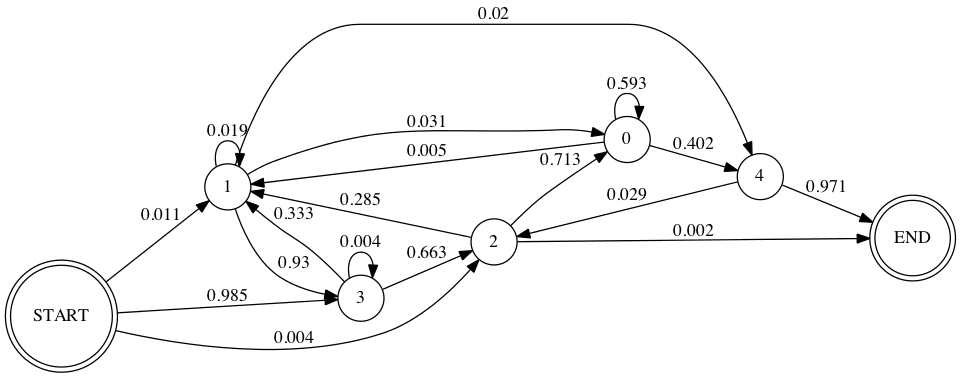
\includegraphics[width=1\textwidth]{./figure/HiddenMarkov5.png}
 \caption{trnasition graphic model with 5 hidden state: In this figure, we ignore transition probability lower than $10 ^{-4}$ and we can see that some of the transition between states are ignorable, which is a indication that hidden states do have their own iterpretations}
 \end{figure}
\paragraph{} First, as we increase the number of hidden states, the quality of the generated sentences is increasing. We interpret this phenomenon as such: when the number of hidden states is small, some very different word have to be put into the same state. When generating sequences, not all word pairs under consecutive hidden states are meaningful(actually only a small number of pairs are). If we increase the number of hidden states to be almost equal to the number of words in the corpus, then usual word pairs are easily captured. Another benefit of increasing number of hidden states is that the sentence length is tending to have less variation. We randomly generate 1000 sentences when the number of hidden states equals 5, 100 and 1000 and plot the generated sentence length distribution. We find that as the number hidden states increases, the sentence length is more centered around 8-9, which is the typical length of a line in a sonnet.
%\begin{figure}[ht]
%\centering
%\begin{minipage}[b]{0.45\linewidth}
%	\centering
%  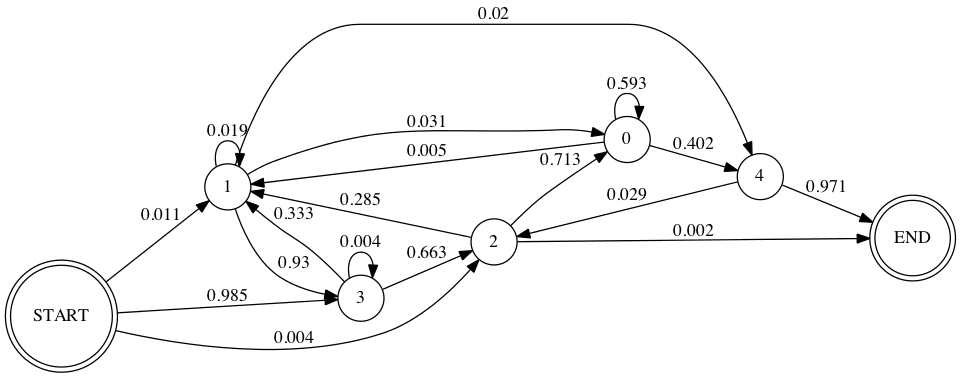
\includegraphics[width=0.6\linewidth]{./figure/HiddenMarkov5.png}
%  \caption{Happy Smiley}
%  \label{fig:minipage1}
%\end{minipage}
%\quad
%\begin{minipage}[b]{0.45\linewidth}
%	\centering
%  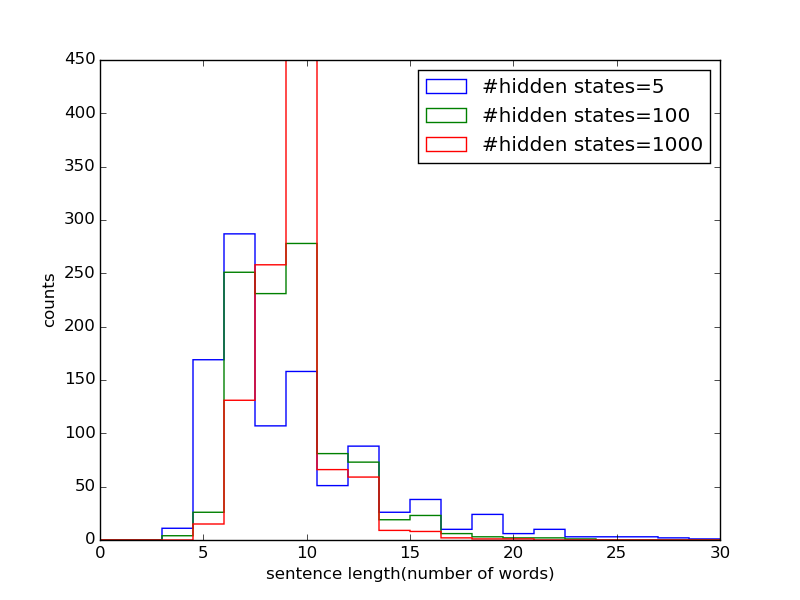
\includegraphics[width=0.6\linewidth]{./figure/hiddenstate_len_distri.png}
%  \caption{Sad Smiley}
%  \label{fig:minipage2}
%\end{minipage}
%\end{figure}

 \begin{figure}[h!]
 \centering
 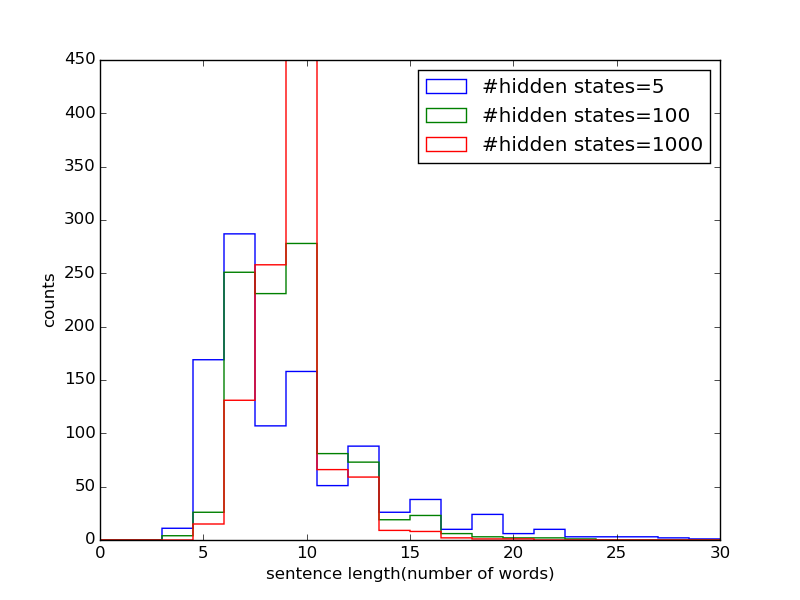
\includegraphics[width=0.5\textwidth]{./figure/hiddenstate_len_distri.png}
 \caption{Sentence length distribution with different number of hidden states. When number of hidden states=1000, the length of the sentences are centered arount 8-9.}
 \end{figure}
\vspace{5pt}
\subsection{Interpreting the hidden states}
\vspace{5pt}

\paragraph{} Here we also present our findings about the interpretations of the hidden states.
The hidden states should bear some meanings in a sense that words likely to be emitted from the same hidden states should more or less share some common features. We find that the words pertaining to different hidden state may have difference in their part of speech tag, syllables and positions in a sentence.

For simplicity, in the following discussion we are always using 5 hidden states example.  We plot the transition diagram of the 5 hidden states. From that we can see there is a close connection between hidden states and the position in a sentence.
For each sentence in the training corpus, we use Viterbi algorithm to find the most likely corresponding hidden state sequences.We count how many times a certain state appears in a certain position of a sentence.  We plot out the distribution of the occurring position of the 5 hidden states in those maximum likelihood sequences. 
It is clear that each of the 5 hidden states have peaks in different positions of a sentence. State 2 is most likely to be the starting word of a sentence while state 4 end of a sentence.
 \begin{wrapfigure}[20]{l}{0.5\textwidth}
 %\begin{center}
 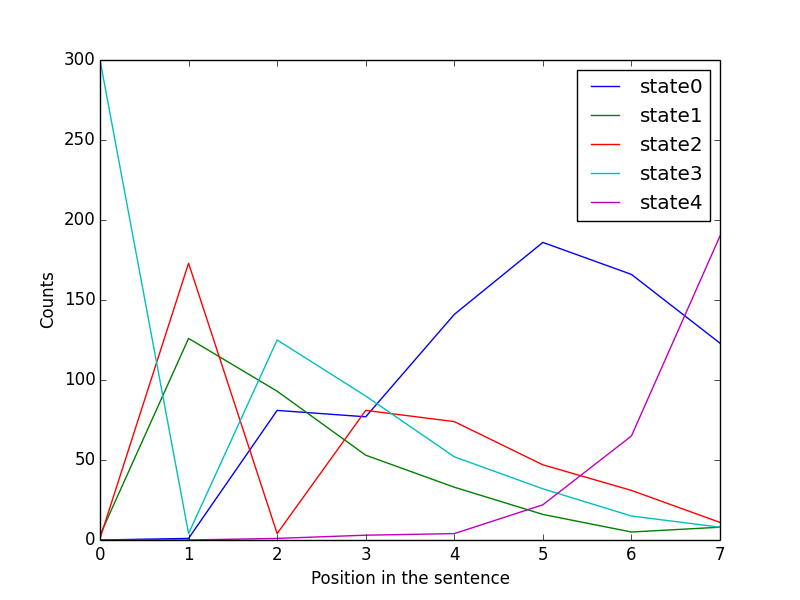
\includegraphics[width=0.5\textwidth]{./figure/hiddenstates_position_in_the_sentence.png}
 \caption{The distribution of different hidden states showing up at different positions in a sentence. Here we assume that a sentence is made of 8 words. If the actual length is greater than 8, then the later positions are also categorized as position 7.\label{fig:position}}
 %\end{center}
\end{wrapfigure}
\section*{}
\vspace{10pt}
\paragraph{}
Words pertaining to the 5 hidden states also have different distribution in their corresponding part of speech tags.  For each sentence in the corpus, we use the part of speech tags marking tools provided by NLTK package to see the part of speech tag each hidden state is corresponding to and then make a histogram of how many times a hidden states appears in a sentence as a noun, verb, adj, adv,. We find that state 1 is most likely to appear as a noun while state 2 is more likely to appear as verb. Conjunction words like \textbf{'and'}, \textbf{'or'} are more likely to be under state 2 and 3 while state 4, usually at the end of a sentence, is limited to noun and verb. \ref{fig:position} illusstrates the relationship between hidden states and positions in a sentence.
\\
\\
 \begin{figure}[h]
 \centering
 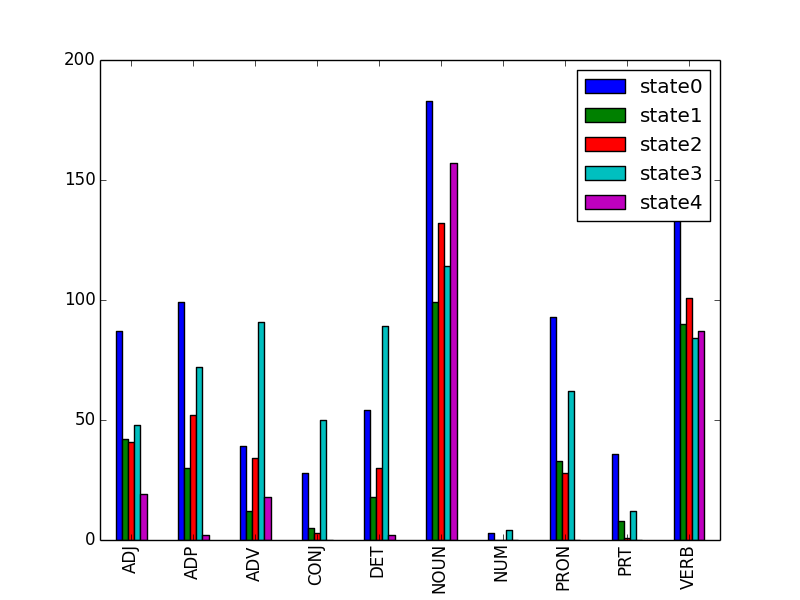
\includegraphics[width=0.5\textwidth]{./figure/hiddenstate_partofspeechtag.png}
 \caption{Statistics of corresponding part of speech tag for each state in the maximum likelyhood sequence given by viterbi algorithm}
 \end{figure}
\paragraph{}
%\vspace{35pt}
\section*{}
The number of syllables in each state is not so different. We choose the most probable 200 word that is emitted by each of the 5 states and count their number of syllables. The emitting probability has been normalized by word frequency. We didn’t find significant differences between each state. 


\paragraph{}
To make a conclusion, the five states has clear meaning representing the position in a sentence. It also has some relationship to the part of speech tags. But the two effects are not independent. It might be that a certain state have to be the first state in a sentence so that it prefers some part of speech tags rather than others. In this study, the hidden state doesn't seem to bear sentimental meanings because the corpus is so small and most words appear only once. So there is no way to tell their sentimental polarity. If we have a larger corpus, by using more hidden states, we could dig out more sentimental meanings. 
%\newline
 \begin{wrapfigure}[16]{r}{0.5\textwidth}
 \centering
 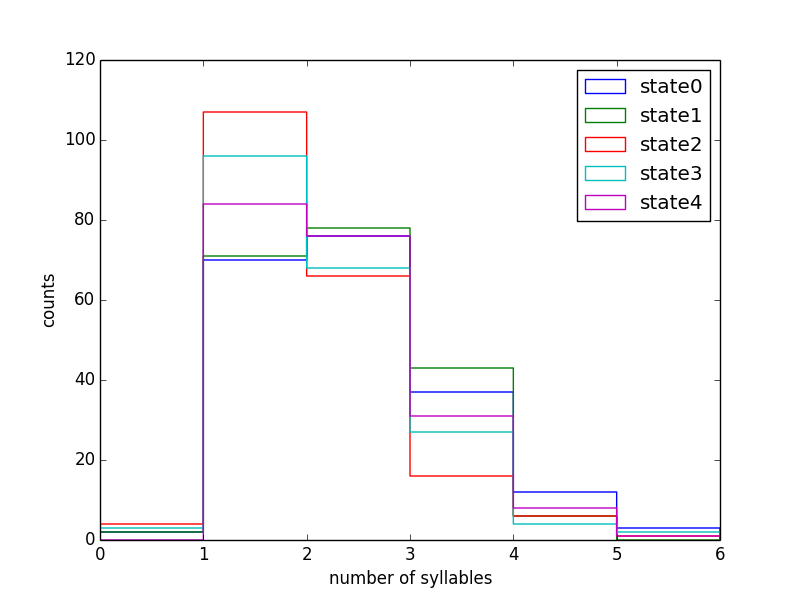
\includegraphics[width=0.5\textwidth]{./figure/numberofsyllablesinstates.png}
 \caption{Number of syllables in the most probable 200 emitting words for each hidden state.}
\end{wrapfigure}


\section{Poetry Generation}
%
\paragraph{}\label{sec:syllablecount}
We present results from the models we worked on in this project. As stated above, we do counting in the poetry generation to make sure that each line in our poem consists of 10 syallables.That is to say, we actually generation our poetry line by line, at each position of line, we repeated generate lines until we get a 10-syllable line: we only took our pick of lines with 10 syllables. In counting the syllables, we use dictionary from \textit{NLTK} and package \textit{PyHyphen} to break words into syllables, we did not truncate lines during the counting, so each line is supposed to end up in the \textit{END} state (this is the same for both Hidden Markov Model and Hidden Markov Model). We only took our pick at sentence level.
\subsubsection{1st Hidden Markov Model}

\subsubsection{2nd order Markov Chain Model}
\paragraph{}
Here is a poem we generated from our reversed-trained 2nd order Markov Model, with automatically marked punctuation, we name it \textbf{'Beauty and Love'}:
\renewcommand{\poemtoc}{subsection}
\poemtitle{Hope or Fear?}
\settowidth{\versewidth}{Thy proud hearts slave and vassal wretch to be?}
\begin{verse}[\versewidth]
They know what beauty, is see where it lies,\\
For that deep wound it gives my friend and me,\\
But tis my heart that loves what they despise,\\
So you oer green my bad my good allow:\\
The mortal moon hath her eclipse endured,\\
And given to time your own dear purchased right;\\
Incertainties now crown themselves assured,\\
On both sides thus is simple truth suppressed.\\
Thou hast passed by the ambush of young days,\\
And all things turns, to fair that eyes can see,\\
Yet this thy praise cannot be so thy praise,\\
Thy proud hearts slave and vassal wretch to be?\\
\vin Thine by thy beauty tempting her to thee,\\
\vin  So long lives this and this shall ever be.\\
\end{verse}

\section{Additional researches that we have worked on}
%
\subsection{Rhyme}\label{sec:rhymedict}
The naive approach to generate poems does not honor the rhyme pattern in the Shakespear's sonnets. However, it is actually not difficult to introduce rhyme in our group-based poem generating algorithms. There are two steps to generate poems with rhymes: first, build a rhyming dictionary; second, seed the end of the line with words that rhyme, and then do HMM generation in the reverse direction.

To build a rhyming dictionary, we pick out the last words of pair of rhyming lines. If these two words rhyme, we add it to the rhyming dictionary. For example, ``increase" and ``decease" rhyme with the same phonetic ``IY-S" (\texttt{cmudict} phonetic form), and thus we generate an phonetic item ``IY-S" in the rhyming dictionary with two words ``increase" and ``decease". In Sonnet 11, we find another pair ``increase" and ``cease" also rhyme with ``IY-S". Then, we add ``cease" into the item ``IY-S". Sometimes, the last words of pair of rhyming lines do not rhyme, like ``die" and ``memory". In this case, we only check these two words separately whether they can be added into some existing phonetic item. For example, ``die" can be added into the phonetic item ``AY" and ``memory" can be added into the phonetic item ``IY". After traversing all the rhyming lines twice, we build a rhyming dictionary for each corpus. 

We combine the \textit{NLTK} package and the RhymeBrain website~\url{http://rhymebrain.com/en} to identify whether two words rhyme or not and the phonetic they rhyme. For the word which exists in \texttt{cmudict} (in \textit{NLTK}), we use \textit{NLTK} to get its phonetics. For example, 
\begin{lstlisting}
>>> phondict = nltk.corpus.cmudict.dict()
>>> phondict['increase']
[[u'IH0', u'N', u'K', u'R', u'IY1', u'S'], [u'IH1', u'N', u'K', u'R', u'IY2', u'S']]
\end{lstlisting}
If either of the pronunciation rhymes with other word, like ``cease", we think that these two words rhyme. For the word which does not exists in \texttt{cmudict}, our script \textit{automatically} picks an auxiliary word which rhyme with this word from the RhymeBrain website~\url{http://rhymebrain.com/en}, and use the phonetics of the auxiliary word to analyze the rhyme. For example, ``fulfil" does not exists in \texttt{cmudict}. Our script will go to the RhymeBrain website and pick the word ``foothill". Then we use 
\begin{lstlisting}
>>> phondict['foothill']
[[u'F', u'UH1', u'T', u'HH', u'IH2', u'L']]
\end{lstlisting}
to analyze whether ``fulfil" and ``will" rhyme, and the answer is yes!

In this case, we train the HMM or 2rd-order Markov model in the reverse direction. To do this, we only need to reverse every line in the input corpus. To generate a poem, we first seed the end of the line with words that rhyme, and then generate lines with the reverse-direction-trained model. \textit{The following are several rhyming lines generated by trained HMM for \texttt{groupG} with number of hidden state 80.}
\settowidth{\versewidth}{even  see  shall  accessary  used  must  find  and  herself  enfeebled  mine  it}
\begin{verse}[\versewidth]
 as  with  proves  replete  in  thee  writ \\
 even  see  shall  accessary  used  must  find  and  herself  enfeebled  mine  it  \\
 she  this  and  thee  praise  \\
 then  love  away  night  seat  is  one  days  \\
 this  even  had  in  lived  their  young  part  \\
 yet  subjects  knife  what  right  winter  thee  heart  \\
 and  thou  feelst  find  bear  wretchcd  your  store  line  \\
 that  other  not  may  it  of  shows  this  mine  in  writ  mine  \\
 pity  mayst  be  you  made  to  praise  best  \\
 the  thee  be  him  and  length  time  thou  am  still  breast  
\end{verse}
We can see that the lines alway rhyme, but the number of syllables varies a lot.

\subsection{Controlling the total number of syllables in a line}\label{sec:syllablecount}
There are several ways to control the total number of syllables in each line and ideally to make it exactly 10. We take a very simple approach to do this: repeatedly generating lines until the total number of syllables is 10. Sometimes, it takes a long time to get a line with exactly 10 syllables. Therefore, we randomly generate at most 50 lines, and keep the line whose total number of syllables is closest to 10.

To count the total number of syllables in each line, we need to count the number of syllables in each word. We combine the \textit{NLTK} package, the \textit{PyHyphen} package and our own-written function \texttt{count\_syllables()} to count the number of syllables in each word as accurate as possible. If a word is in \texttt{cmudict}, the \textit{NLTK} gives us the right answer. For examples, ``increase" has 2 syllables according to \texttt{cmudict}. If a word is not in \texttt{cmudict}, we use \textit{PyHyphen} to count the syllables. For example,
\begin{lstlisting}
In[4]: from hyphen import Hyphenator
In[5]:  h_en = Hyphenator('en_US')
In[6]: len(h_en.syllables(unicode('fulfil')))
Out[6]: 2
In[7]: len(h_en.syllables(unicode('air')))
Out[7]: 0
\end{lstlisting}
We can see that the \textit{PyHyphen} package is not so accurate to identify the number of syllables in a word. Therefore, we also write our own function \texttt{count\_syllables()} (see file \texttt{countvowel.py}) to correct possible mistakes made by the \textit{PyHyphen} package.

With this approach to control the total number of syllables in a line, we get rhyming lines all of which have total number of syllables nearly 10. \textit{The following are several rhyming lines generated by trained 2rd-order Markov model for \texttt{groupG}.}
\settowidth{\versewidth}{even  see  shall  accessary  used  must  find  and  herself  enfeebled  mine  it}
\begin{verse}[\versewidth]
 which  die  for  goodness  who  have  lived  for  crime \\
 but  were  some  child  of  yours  alive  that  time \\
 to  give  back  again  and  straight  grow  sad \\
 this  told  joy  but  then  no  longer  glad \\
 lo  thus  by  day  my  limbs  by  night  my  mind \\
 for  thee  and  for  my  name  thy  love  and  am  blind \\
 think  all  but  one  and  me  most  wretchcd  make \\
 till  then  not  show  my  head  where  thou  mayst  take \\
 so  till  the  judgment  that  your  self  arise \\
 so  long  lives  this  and  dwell  in  lovers  eyes
\end{verse}
We can see that the lines alway rhyme, and the total number of syllables in each line is nearly 10.


\subsection{Incorporating additional texts} \label{sec:additionaltext}
Our framework enables us to train our models with additional texts. We include all 139 of Spenser's sonnets in our training datasets. With the same process, i.e., pre-processing, rhyme dictionary learning, model training (for both HMM and 2rd-order Markov model), we can easily get models which have a larger dictionary. The training time nearly get doubled because we have nearly double sized training data. The following is one poem from our trained 2rd-order Markov model, with rhyming and controlling-the-total-number-of-syllables.
\settowidth{\versewidth}{even  see  shall  accessary  used  must  find  and  herself  enfeebled  mine  it}
\begin{verse}[\versewidth]
 the  dedicated  words  which  writers  use \\
 to  new  found  methods  and  to  compounds  strange \\
 as  fast  as  thou  art  too  dear  for  my  muse \\
 so  far  from  variation  or  quick  change \\
 reserve  them  for  my  love  doth  well  denote \\
 or  from  their  proud  lap  pluck  them  where  they  grew \\
 if  that  be  fair  whereon  my  false  eyes  dote \\
 at  wondrous  sight  of  so  celestial  hew \\
 prison  my  heart  with  silence  secretly \\
 and  sweets  grown  common  lose  their  dear  delight \\
 but  rising  at  thy  name  doth  point  out  thee \\
 than  when  her  mournful  hymns  did  hush  the  night \\
 \vin so  return  rebuked  to  my  content \\
 \vin that  it  hereafter  may  you  not  repent
\end{verse}

After examination, we find that the first line ``the  dedicated  words  which  writers  use" is actually borrowed from Shakespear sonnet 82, and the eighth line ``at  wondrous  sight  of  so  celestial  hew" is borrowed from Spenser sonnet 3. Other lines are not directly borrowed from either of them, but are kind of mixture of them. For example, the third line "as  fast  as  thou  art  too  dear  for  my  muse" is a combination of  ``As fast as thou shalt wane so fast thou grow'st" from Shakespere sonnet 11 and ``So oft have I invoked thee for my muse" from Shakespere sonnet 78. By introducing additional texts (spenser's poems), we get more variations in the poems we generate.

\subsection{Adding punctuations}\label{sec:punctuations}



%\begin{enumerate}
%\item Briefly introduce all the algorithms you tried to implement
%\item Elaborate on the specifics of each algorithm you implemented, and the performance achieved.
%\begin{enumerate}
%\item algorithm1
%\item algorithm2
%\item $\cdots$
%\end{enumerate}
%\end{enumerate}


%\section{Model Selection}
%Describe the steps you took to pick your final model, such as cross-validation.

\section{A reference for our document}
%


\section{Conclusion}
%
\paragraph{}
In this project, we trained \textbf{Hidden Markov Models (HMMs)} and \textbf{2nd-order Markov Models} for poem generation.

Due to the clear rhyme pattern in Shakespeare's sonnets, the basic strategy in our model training is to train multiple models for different part of the poem. We tokenize the words as features in each group and run the EM algorithm with different number of hidden states to train the HMMs. Looking into the HHMs with 5 hidden states, we are able to find a clear relationship between the position of words and hidden states they correspond to. The speech tags of words also show a strong correlation with the 5 hidden states. Since HHMs is a probabilistic model, we are able to generate poems by the HHMs we trained. 

After examining the HHMs with different number of hidden states, we found that the more hidden states the HHM has, the more meaningful sentences it can generate. Due to this observation, we decided to also train Markov models. We tried the standard (first-order) Markov model and the second-order Markov model and found that the second-order Markov model works very well to learn short phrases and to generate meaningful sentences. However, we also noticed that sometimes the second-order Markov model just \textit{``borrows"} sentences from the training dataset. But what the 2nd order Markov Model is trying to do is \textbf{capturing the meaning}, so each verse generated by it reads comparatively more reasonable. We see, because of this, 2nd Order Markov Model will generate jointed sentences like \textbf{Men call you fair}, and \textbf{you do write}'. This \textit{``borrowing''} phenomena is mainly why we think higher order may not perform much better than the second order, in the poetry language, especially,we have usually taken 2 word as a phrase. And if the order of the model is too high, actually we may generate a whole line from the original data set, and that is not what we are expecting. 

The naive approach to train both the HHMs and the 2nd-order Markov models honors neither the rhyme pattern nor the iambic pentameter in Shakespeare's sonnets. To generate poems whose lines rhyme, we first use the \textit{NLTK} package and the \textit{RhymeBrain} website~\url{http://rhymebrain.com/en} to build a \textbf{rhyming dictionary}, and then generate each line in the reverse direction with pre-sampled ending words that rhyme. To honor the iambic pentameter, we try to generate lines with total number of syllables as close to 10 as possible. To achieve this goal, we simply keep generating lines until we get a line with exactly 10 syllables. With these additional modifications, we can finally generate Shakespeare-style poems with both the HHMs and the 2nd-order Markov models. Our framework enables us to train our models with additional texts. We include all 139 of Spenser's sonnets in our training dataset and get models with bigger dictionary and generate poems with more variations. 

Since we generate rhyming lines for each group independently, our models \textit{can't} keep a unified topic across all the 14 lines. Although every line makes some sense separately, the whole poem sounds like a drunk Shakespeare who randomly jumps from one topic to another. If we have more time on this project, we may introduce some mechanism to unify all the lines with a common topic. To achieve this goal, one possible solution is to first train a topic model from the dataset. To generate a poem, one can first choose a topic and sample key words from this topic for each line. Finally, one can generate each line with the given key words with either the HMMs or the 2nd-order Markov models. In this way, the given key words in each line can unify all the lines together. 

\end{document}
